\documentclass[fleqn]{article}
\usepackage[nodisplayskipstretch]{setspace}
\usepackage{amsmath, nccmath, bm}
\usepackage{amssymb}
\usepackage{enumitem}
\usepackage{etoolbox}
\usepackage{graphicx}
\usepackage{float}
\usepackage{changepage}
\usepackage{environ,capt-of}

\let\oldfigure\figure% Store original figure float environment
\let\endoldfigure\endfigure
\RenewEnviron{figure}[1][H]{% Update figure environment
  %\par\vspace{\intextsep}% Assume in-text placement, so insert appropriate vertical spacing
  \noindent
  % \patchcmd{<cmd>}{<search>}{<replace>}{<success>}{<failure>}
  \patchcmd{\BODY}{\caption}{\captionof{figure}}{}{}% Replace \caption with \captionof{figure} inside \BODY
  % Set "figure"
  \begin{minipage}{\linewidth}
    \BODY
  \end{minipage}
  %\par\vspace{\intextsep}% Assume in-text placement, so insert appropriate vertical spacing
}

\newcommand{\zerodisplayskip}{
	\setlength{\abovedisplayskip}{0pt}%
	\setlength{\belowdisplayskip}{0pt}%
	\setlength{\abovedisplayshortskip}{0pt}%
	\setlength{\belowdisplayshortskip}{0pt}%
	\setlength{\mathindent}{0pt}}
	
\title{Homework 4}
\author{Owen Sowatzke}
\date{March 29, 2024}

\begin{document}

	\offinterlineskip
	\setlength{\lineskip}{12pt}
	\zerodisplayskip
	\maketitle
	
	\begin{enumerate}
		\item Show that if the activation function of the hidden layer is linear, a three layer network is equivalent to a two layer one.
		
		\begin{figure}[H]
			\centerline{\fbox{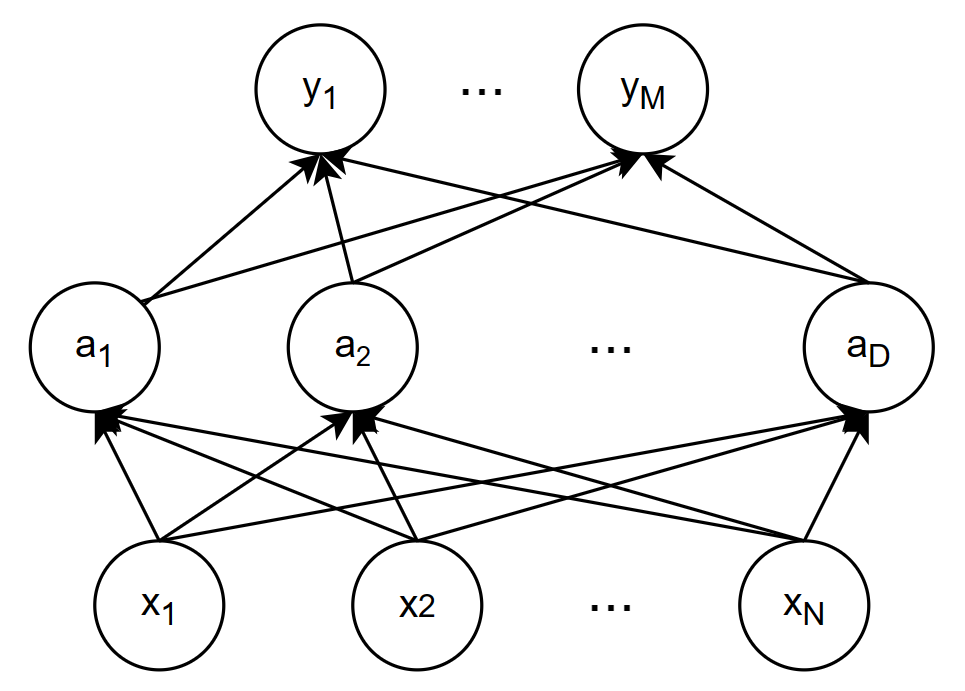
\includegraphics[width=0.4\textwidth]{neural_network_3_layer.png}}}
			\caption{3-Layer Neural Network}
			\label{neural_network_3_layer}
		\end{figure}
	
		The output of the neural network is given by $\mathbf{y} = Q_1(\mathbf{F_1}Q_2(\mathbf{F_2}\mathbf{x}))$ where $Q_2(\boldsymbol{\alpha})$ is the activation function of the hidden layer.
		
		If $Q_2(\boldsymbol{\alpha})$ is linear it can be rewritten as $\mathbf{H}\boldsymbol{\alpha}$. If we substitute this expression for the hidden layer into the above formula, we get the following:
		
		$\mathbf{y} = Q_1(\mathbf{F_1}Q_2(\mathbf{F_2}\mathbf{x})) = Q_1(\mathbf{F_1H(F_2\mathbf{x})}) = Q_1(\mathbf{F_1HF_2x}) = Q_1(\mathbf{Ax})$
		
		where $\mathbf{A} = \mathbf{F_1HF_2}$.
		
		Therefore, the neural network is equivalent to two-layer neural network.
		
		\begin{figure}[H]
			\centerline{\fbox{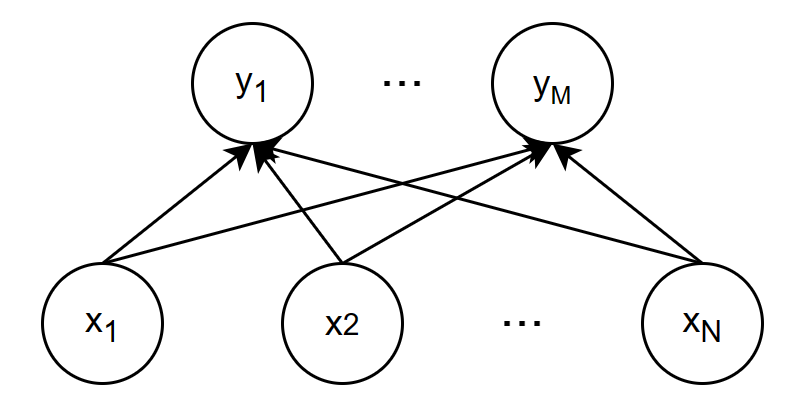
\includegraphics[width=0.4\textwidth]{neural_network_2_layer.png}}}
			\caption{2-Layer Neural Network}
			\label{neural_network_2_layer}
		\end{figure}
		
		\item Assume that a network produces the output $y_i$ in response to the i-th training image from class 1, and the output $x_i$ in response to the i-th training image from class 2. We wish to train the network to maximize the cost function $J(\text{net}) = \frac{\sum_{i=1}^{N}{y_i^2}}{\sum_{i=1}^{N}{x_i^2}}$. Derive the gradient for this cost function and describe how the network updates might be made using batch training and a single image at a time.
		
		We can re-express the gradient in matrix-vector notation as follows:
		
		\begin{equation*}
			J(\text{net}) = \frac{\mathbf{y}^T\mathbf{y}}{\mathbf{x}^T\mathbf{x}}
		\end{equation*}
		
		where $\mathbf{x} = \begin{bmatrix}x_1 & x_2 & \cdots & x_N \end{bmatrix}^T$ and $\mathbf{y} = \begin{bmatrix}y_1 & y_2 & \cdots & y_N \end{bmatrix}^T$
		
		\begin{equation*}
			\nabla_{\mathbf{y}}{J} = \frac{2\mathbf{y}}{\mathbf{x}^T\mathbf{x}} \ \text{and}\ \nabla_{\mathbf{x}}{J} = -\frac{2\mathbf{x}\mathbf{y}^T\mathbf{y}}{(\mathbf{x}^T\mathbf{x})^2}
		\end{equation*}
		
		Define $\mathbf{z} = \begin{bmatrix} \mathbf{y} \\ \mathbf{x} \end{bmatrix}$. Then, we can express $\nabla_{\mathbf{z}}{J}$ as follows:
		
		\begin{equation*}
			\nabla_{\mathbf{z}}{J} = \begin{bmatrix}
				\frac{2\mathbf{y}}{\mathbf{x}^T\mathbf{x}} \\[3pt]
				-\frac{2\mathbf{x}\mathbf{y}^T\mathbf{y}}{(\mathbf{x}^T\mathbf{x})^2}
			\end{bmatrix}
		\end{equation*}
		
		In other words
		
		\begin{equation*}
			\frac{\partial{J}}{\partial{y_i}} = \frac{2y_i}{\sum_{i=1}^{N}x_i^2}\ \text{and}\ \frac{\partial{J}}{\partial{x_i}} = -\frac{2x_i\sum_{i=1}^{N}y_i^2}{\left(\sum_{i=1}^{N}x_i^2\right)^2}
		\end{equation*}
	\end{enumerate}
\end{document}